%% =======================================================
%% Actividad 22: Modelos de predicción
%%
%% Compilar desde actividades/: ./compilar.sh act22
%% Las figuras de img/ se generan con: python act22.py
%% =======================================================

%% ---- CONFIGURACIÓN ------------------------

\documentclass[11pt,letterpaper]{article}

\usepackage[indice]{tecnm}
\usepackage[T1]{fontenc}
\usepackage{amsmath}
\usepackage{xcolor}
\usepackage[most]{tcolorbox} % Carga tcolorbox con soporte para listings y saltos de página
\tcbuselibrary{listings, skins, breakable}
\setlength{\emergencystretch}{3em} % Evita líneas desbordadas por palabras en \texttt

% Paleta de colores (estilo GitHub Light / VS Code)
\definecolor{codebg}{HTML}{F8F9FA}       % Fondo del código
\definecolor{codehead}{HTML}{E9ECEF}     % Fondo de la barra de título
\definecolor{codeborder}{HTML}{CED4DA}   % Borde de la tarjeta
\definecolor{codetitle}{HTML}{212529}    % Texto del título
\definecolor{codekw}{HTML}{0550AE}       % Palabras clave (import, def, for...)
\definecolor{codefunc}{HTML}{8250DF}     % Funciones y métodos (describe, groupby...)
\definecolor{codestr}{HTML}{0A3069}      % Strings
\definecolor{codecomm}{HTML}{6E7781}     % Comentarios
\definecolor{codenum}{HTML}{8C959F}      % Números de línea
\definecolor{codeid}{HTML}{24292F}       % Texto general

% Configuración base de listings
\lstdefinestyle{pythonestilo}{
  language=Python,
  basicstyle=\ttfamily\footnotesize\color{codeid},
  keywordstyle=\color{codekw}\bfseries,
  keywordstyle=[2]\color{codefunc}, % Estilo secundario para métodos de datos
  stringstyle=\color{teal!80!black},
  commentstyle=\color{codecomm}\itshape,
  morekeywords={as, True, False, None, with, yield, lambda},
  morekeywords=[2]{read_csv, RandomForestRegressor, LinearRegression, StandardScaler, KFold, PredefinedSplit, LeaveOneOut, cross_val_predict, train_test_split, mean_absolute_error, mean_squared_error, r2_score, make_pipeline, fit, predict, default_rng, groupby, ngroup, print, len, sum, max, DataFrame, Series, value_counts, reindex, mean, std, var, randint, normal, seed, cumsum, poisson, binom, pmf, norm, fit, kde, bincount, linspace, train_test_split, make_blobs, GaussianNB, chisquare, pdf, cdf, hist, bar, plot, axhline, axvline, fill_between, subplots, figure, concat, nunique, load_iris, diff, sort, unique},
  numbers=left,
  numberstyle=\tiny\ttfamily\color{codenum},
  stepnumber=1,
  numbersep=10pt,
  showstringspaces=false,
  morestring=[b]{"""},
  tabsize=4,
  breaklines=true,
  breakatwhitespace=true,
  columns=flexible,
  keepspaces=true,
  literate=
    {á}{{\'a}}1 {é}{{\'e}}1 {í}{{\'i}}1 {ó}{{\'o}}1 {ú}{{\'u}}1
    {Á}{{\'A}}1 {É}{{\'E}}1 {Í}{{\'I}}1 {Ó}{{\'O}}1 {Ú}{{\'U}}1
    {ñ}{{\~n}}1 {Ñ}{{\~N}}1 {¿}{{?`}}1 {¡}{{!`}}1 {°}{{$^\circ$}}1
}

% Definición del entorno personalizado \begin{codigo}{Título}{etiqueta}
% \newtcblisting[auto counter, number within=section]{codigo}[2][]{
\newtcblisting[auto counter]{codigo}[2][]{
  listing only,
  breakable,                    % Permite que el bloque se divida si pasa de página
  enhanced,
  colback=codebg,
  colframe=codeborder,
  colbacktitle=codehead,
  coltitle=codetitle,
  fonttitle=\bfseries\small\sffamily,
  boxrule=0.6pt,
  arc=4pt,                      % Bordes redondeados
  left=20pt,                    % Espacio izquierdo para los números de línea
  right=8pt,
  top=6pt,
  bottom=6pt,
  toptitle=4pt,
  bottomtitle=4pt,
  before skip=12pt,
  after skip=12pt,
  listing options={style=pythonestilo},
  title={Código \thetcbcounter: #2},
  #1
}

% Paleta para salida de consola (estilo terminal limpia)
\definecolor{termbg}{HTML}{212529}      % Fondo oscuro tipo terminal
\definecolor{termhead}{HTML}{343A40}    % Barra superior
\definecolor{termtext}{HTML}{F8F9FA}    % Texto claro de alta legibilidad
\definecolor{termborder}{HTML}{495057}  % Borde

% Entorno \begin{consola}[label=out:iris]{Título}
\newtcblisting[auto counter]{consola}[2][]{
  listing only,
  breakable,
  colback=termbg,
  colframe=termborder,
  colbacktitle=termhead,
  coltitle=termtext,
  colupper=termtext,
  fonttitle=\bfseries\small\sffamily,
  boxrule=0.6pt,
  arc=4pt,
  left=8pt,
  right=8pt,
  top=6pt,
  bottom=6pt,
  toptitle=4pt,
  bottomtitle=4pt,
  before skip=12pt,
  after skip=12pt,
  listing options={
    basicstyle=\ttfamily\scriptsize\color{termtext}, % \scriptsize evita que las tablas de Pandas se partan de línea
    breaklines=true,
    columns=fixed,        % Mantiene alineadas las columnas de Pandas
    keepspaces=true,
    showstringspaces=false,
    literate=
      {á}{{\'a}}1 {é}{{\'e}}1 {í}{{\'i}}1 {ó}{{\'o}}1 {ú}{{\'u}}1
      {Á}{{\'A}}1 {É}{{\'E}}1 {Í}{{\'I}}1 {Ó}{{\'O}}1 {Ú}{{\'U}}1
      {ñ}{{\~n}}1 {Ñ}{{\~N}}1 {°}{{$^\circ$}}1
  },
  title={Salida \thetcbcounter: #2},
  #1
}

%% ---- DATOS DE LA MATERIA ------------------------

\materia{Modelos Estadísticos para el Aprendizaje \\ Automático y Ciencia de Datos}
\actividad{Tema 3.3 Validación Estadística de Modelos de Aprendizaje Automático \\ Actividad 22 - Modelos de predicción}

\profesor{Dr. José Ismael Ojeda Campaña}
%\fecha{15 de octubre de 2026}    % opcional; por defecto es la fecha de hoy

\begin{document}
\portada
\indicegeneral

%% ---- CONTENIDO ---------------------------------

\section{Introducción}

Cuando un modelo no clasifica sino que predice un valor numérico, las métricas de un clasificador (exactitud, sensibilidad, etc.) dejan de ser adecuadas y se deben usar métricas de bondad y ajuste \parencite{tecnm2026_tema33}. Además, la confiabilidad de cualquier métrica depende de cómo se partieron los datos entre entrenamiento y prueba, y de que esa partición sea apropiada a la cantidad y la estructura de los datos \parencite{tecnm2026_tema33}.

En esta actividad se desarrolla un modelo de regresión sobre un conjunto de datos público del repositorio UCI, el ruido aerodinámico de perfiles alares \parencite{brooks1989}. Se comparan una regresión lineal y un bosque aleatorio con cuatro métodos de partición, se calculan las métricas del tema (MAE, MSE, RMSE y $R^2$) y se discute su efectividad y la validez de los resultados, incluyendo un problema de la estructura de los datos que hace optimistas algunas estimaciones. El script genera automáticamente las tablas y un resumen del análisis.

\section{Marco conceptual}

\subsection{Métricas de bondad y ajuste de un regresor}

Las métricas más comunes para medir la efectividad de un regresor son el error absoluto medio (MAE), el error cuadrático medio (MSE), su raíz (RMSE) y el coeficiente de determinación $R^2$ \parencite{tecnm2026_tema33}. Con $y_i$ la observación, $\hat{y}_i$ la predicción, $\bar{y}$ la media de las observaciones y $N$ el número de datos evaluados:
\begin{align*}
\text{MAE} &= \frac{1}{N}\sum_{i=1}^{N} |\hat{y}_i - y_i|, &
\text{MSE} &= \frac{1}{N}\sum_{i=1}^{N} (\hat{y}_i - y_i)^2, &
\text{RMSE} &= \sqrt{\text{MSE}}, &
R^2 &= 1 - \frac{\sum_i (y_i - \hat{y}_i)^2}{\sum_i (y_i - \bar{y})^2}.
\end{align*}
Estas métricas indican qué tanto se ajustan las predicciones a los valores reales \parencite{tecnm2026_tema33}. Las fórmulas del documento del tema aparecen con un factor $1/(2N)$ en el MAE y el MSE; aquí se usan las definiciones estándar con $1/N$, que dan el error promedio en las unidades de la variable (MAE y RMSE) o en su cuadrado (MSE).

\subsection{Métodos de partición}

El hold-out divide aleatoriamente el conjunto en entrenamiento y prueba (por ejemplo 80\,\%/20\,\% o 70\,\%/30\,\%) y se usa cuando hay datos suficientes, e incluso podría asumirse la independencia de las observaciones. Cuando los datos no bastan se usan alternativas como la validación cruzada de $k$ particiones y leave-one-out (con $k$ igual al número de instancias), en las que no se puede garantizar la independencia y por eso no se emplean con pruebas paramétricas \parencite{tecnm2026_tema33}.

\section{Descripción de la actividad}

\textbf{Objetivo:} Desarrollar un modelo de regresión y aplicar las métricas de evaluación estudiadas en este tema, así como los métodos de partición más apropiados \parencite{tecnm2026_tema33}.

\begin{description}
    \item[Tarea 1: Dataset, partición y modelo.] Identificar un dataset público, a) identificar la técnica de partición más adecuada y b) construir y entrenar el modelo.
    \item[Tarea 2: Comparación de resultados.] Calcular las métricas de bondad y ajuste del tema y compararlas.
    \item[Tarea 3: Análisis de resultados.] Discutir la efectividad de las métricas y del método de partición, aportando un punto de vista sobre la validez de los resultados.
\end{description}

Los entregables son este reporte en PDF y el script \texttt{act22.py}, que realiza el análisis completo y genera reportes automáticos.

\section{Desarrollo}

El script utiliza \texttt{numpy}, \texttt{pandas}, \texttt{scikit-learn} y \texttt{matplotlib}. Descarga los datos del repositorio UCI, por lo que requiere conexión a internet. Los valores de este reporte se obtuvieron con \texttt{scikit-learn} 1.9.1; en otras versiones, sobre todo en los bosques aleatorios, pueden cambiar en la tercera cifra decimal. Las figuras se guardan en la carpeta \texttt{img/}, y las tablas y el reporte automático en \texttt{resultados/}. El Código~\ref{cod:comun} contiene las importaciones, la función \texttt{metricas()}, que calcula MAE, MSE, RMSE y $R^2$, la función \texttt{nuevos\_modelos()}, que define los dos regresores, y la función \texttt{a\_markdown()}, que da formato al reporte automático. El cuaderno interactivo puede consultarse en Google Colab:

\begin{center}
    \url{https://colab.research.google.com/drive/16LZQ9jHlJuqlMnFlMt0WcAQnzvH0vk9G?usp=sharing}
\end{center}

\begin{codigo}[label=cod:comun]{Importaciones, funciones auxiliares y carpetas de salida}
import os

import matplotlib

# En Colab o Jupyter no existe __file__; ahí las figuras también se muestran en pantalla
EN_NOTEBOOK = '__file__' not in globals()
if not EN_NOTEBOOK:
    matplotlib.use('Agg')  # Como script, genera las figuras como archivos PNG sin abrir ventanas

import matplotlib.pyplot as plt
import numpy as np
import pandas as pd
from sklearn.ensemble import RandomForestRegressor
from sklearn.linear_model import LinearRegression
from sklearn.metrics import mean_absolute_error, mean_squared_error, r2_score
from sklearn.model_selection import (KFold, LeaveOneOut, PredefinedSplit, cross_val_predict,
                                     train_test_split)
from sklearn.pipeline import make_pipeline
from sklearn.preprocessing import StandardScaler

pd.set_option('display.width', 120)
SEMILLA = 42

# Carpetas donde se guardan las figuras del reporte y las tablas del reporte automático
BASE = os.getcwd() if EN_NOTEBOOK else os.path.dirname(os.path.abspath(__file__))
CARPETA_IMG = os.path.join(BASE, 'img')
CARPETA_RES = os.path.join(BASE, 'resultados')
os.makedirs(CARPETA_IMG, exist_ok=True)
os.makedirs(CARPETA_RES, exist_ok=True)


def guardar(nombre):
    """Guarda la figura actual en la carpeta img/ y la muestra si se ejecuta en un notebook."""
    plt.tight_layout()
    plt.savefig(os.path.join(CARPETA_IMG, nombre), dpi=150)
    if EN_NOTEBOOK:
        plt.show()
    plt.close()


def metricas(y_real, y_pred):
    """Métricas de bondad y ajuste del tema 3.3 para un regresor."""
    mse = mean_squared_error(y_real, y_pred)
    return {'MAE': mean_absolute_error(y_real, y_pred), 'MSE': mse,
            'RMSE': np.sqrt(mse), 'R2': r2_score(y_real, y_pred)}


def a_markdown(tabla, indice=True):
    """Convierte un DataFrame en una tabla Markdown (sin depender del paquete tabulate)."""
    tabla = tabla.reset_index() if indice else tabla
    lineas = ['| ' + ' | '.join(str(c) for c in tabla.columns) + ' |',
              '|' + '---|' * len(tabla.columns)]
    for _, fila in tabla.iterrows():
        lineas.append('| ' + ' | '.join(str(v) for v in fila) + ' |')
    return '\n'.join(lineas)


def nuevos_modelos():
    """Dos regresores: uno lineal (referencia) y uno no lineal (bosque aleatorio)."""
    return {'Regresión lineal': make_pipeline(StandardScaler(), LinearRegression()),
            'Bosque aleatorio': RandomForestRegressor(n_estimators=100, random_state=SEMILLA, n_jobs=-1)}
\end{codigo}

\subsection{Datos: selección del conjunto de datos}

Se eligió Airfoil Self-Noise del UCI Machine Learning Repository \parencite{brooks1989}: 1503 ensayos de perfiles alares realizados en un túnel de viento. La variable a predecir es la presión sonora (en decibeles) y las cinco variables predictoras son la frecuencia, el ángulo de ataque, la longitud de la cuerda, la velocidad del flujo y el espesor de desplazamiento del lado de succión. Es un problema de regresión con variables numéricas y sin valores faltantes (Código~\ref{cod:t1}).

\begin{codigo}[label=cod:t1]{Datos: selección del conjunto de datos}
# Airfoil Self-Noise (NASA), del repositorio UCI: ruido aerodinámico de perfiles alares
# medido en túnel de viento. Objetivo: presión sonora (dB) a partir de 5 variables.
URL = 'https://archive.ics.uci.edu/ml/machine-learning-databases/00291/airfoil_self_noise.dat'
columnas = ['frecuencia', 'angulo', 'cuerda', 'velocidad', 'espesor', 'presion_sonora']
datos = pd.read_csv(URL, sep='\t', header=None, names=columnas)
X = datos.drop(columns='presion_sonora')
y = datos['presion_sonora']

print("=== Datos: Airfoil Self-Noise (UCI) ===")
print(f"Instancias: {len(X)}; variables predictoras: {X.shape[1]}; valores faltantes: {int(datos.isna().sum().sum())}")
print(datos.describe().loc[['mean', 'std', 'min', 'max']].round(3).T.to_string())
\end{codigo}

\begin{consola}[label=out:t1]{Ejecución de \texttt{act22.py}: datos}
=== Datos: Airfoil Self-Noise (UCI) ===
Instancias: 1503; variables predictoras: 5; valores faltantes: 0
                    mean       std      min        max
frecuencia      2886.381  3152.573  200.000  20000.000
angulo             6.782     5.918    0.000     22.200
cuerda             0.137     0.094    0.025      0.305
velocidad         50.861    15.573   31.700     71.300
espesor            0.011     0.013    0.000      0.058
presion_sonora   124.836     6.899  103.380    140.987
\end{consola}

La presión sonora tiene media 124.8~dB y desviación estándar 6.9~dB, con valores entre 103.4 y 141.0~dB. Esa desviación es la referencia para juzgar los errores: un modelo que siempre predijera la media tendría un RMSE de 6.9~dB.

\subsection{Tarea 1a: Técnica de partición más adecuada}

Para elegir la partición se revisó primero la estructura de los datos. Cada fila es un ensayo, pero el mismo montaje experimental (misma combinación de ángulo, cuerda, velocidad y espesor) se mide a varias frecuencias. Después se repitieron 30 veces el hold-out 80/20 y la validación cruzada de 10 particiones con semillas distintas, para medir cuánto cambia la estimación según la partición (Código~\ref{cod:t2}).

\begin{codigo}[label=cod:t2]{Tarea 1a: técnica de partición más adecuada}
# Primero se revisa la estructura de los datos: cada fila es un ensayo en el túnel de viento y
# el mismo montaje (ángulo, cuerda, velocidad, espesor) se mide a varias frecuencias.
print("\n=== Tarea 1a: estructura de los datos y técnica de partición ===")
montaje = datos.groupby(['angulo', 'cuerda', 'velocidad', 'espesor']).ngroup()
filas_por_montaje = montaje.value_counts()
print(f"Montajes distintos: {montaje.nunique()}; filas por montaje: mín = {filas_por_montaje.min()}, "
      f"máx = {filas_por_montaje.max()}, media = {filas_por_montaje.mean():.1f}")

# Se repiten hold-out (80/20) y validación cruzada de 10 particiones con semillas distintas para
# medir cuánto cambia la estimación según la partición elegida.
rng = np.random.default_rng(SEMILLA)
N_REP = 30
filas = []
for nombre, modelo in nuevos_modelos().items():
    est_hold, est_cv = [], []
    for _ in range(N_REP):
        semilla = int(rng.integers(1_000_000))
        a, b, c, d = train_test_split(X, y, test_size=0.20, random_state=semilla)
        est_hold.append(metricas(d, modelo.fit(a, c).predict(b)))
        cv = KFold(n_splits=10, shuffle=True, random_state=semilla)
        est_cv.append(metricas(y, cross_val_predict(modelo, X, y, cv=cv)))
    for metodo, est in (('hold-out 80/20', est_hold), ('10-fold', est_cv)):
        est = pd.DataFrame(est)
        filas.append((nombre, metodo, est['RMSE'].mean(), est['RMSE'].std(), est['R2'].mean(), est['R2'].std()))
variabilidad = pd.DataFrame(filas, columns=['modelo', 'método', 'RMSE media', 'RMSE desv.', 'R2 media', 'R2 desv.'])
print(f"Variabilidad en {N_REP} repeticiones con particiones distintas:")
print(variabilidad.round(4).to_string(index=False))
\end{codigo}

\begin{consola}[label=out:t2]{Ejecución de \texttt{act22.py}: Tarea 1a}
=== Tarea 1a: estructura de los datos y técnica de partición ===
Montajes distintos: 106; filas por montaje: mín = 8, máx = 19, media = 14.2
Variabilidad en 30 repeticiones con particiones distintas:
          modelo         método  RMSE media  RMSE desv.  R2 media  R2 desv.
Regresión lineal hold-out 80/20      4.8562      0.1949    0.5085    0.0395
Regresión lineal        10-fold      4.8230      0.0041    0.5109    0.0008
Bosque aleatorio hold-out 80/20      1.7579      0.1134    0.9352    0.0089
Bosque aleatorio        10-fold      1.6671      0.0209    0.9416    0.0015
\end{consola}

Hay 106 montajes distintos, con entre 8 y 19 filas cada uno (14.2 en promedio): las filas de un mismo montaje no son independientes entre sí. Respecto a la estabilidad, el hold-out cambia mucho con la partición: en la regresión lineal el $R^2$ varía con desviación estándar de 0.040 (contra 0.0008 en 10-fold) y en el bosque aleatorio el RMSE tiene desviación estándar de 0.113~dB (contra 0.021~dB en 10-fold). Con 1503 datos, el criterio del tema permitiría un hold-out, pero la validación cruzada de 10 particiones es mucho más estable y usa todos los datos para probar. Leave-one-out no aporta nada con este tamaño y, con el bosque aleatorio, exigiría entrenar 1503 modelos; solo se calculó con la regresión lineal, que es barata. La técnica más adecuada es entonces la validación cruzada de 10 particiones, y por la estructura de los datos se añade una variante que respeta los montajes (10 particiones por grupos), explicada en la Tarea 1b.

\subsection{Tarea 1b: Construcción y entrenamiento de los modelos}

Se entrenaron dos modelos: una regresión lineal con variables estandarizadas, como referencia, y un bosque aleatorio de 100 árboles, que captura relaciones no lineales. Cada modelo se evaluó con cuatro particiones: hold-out 80/20 (1202 datos de entrenamiento y 301 de prueba), 10-fold aleatorio, leave-one-out (solo regresión lineal) y 10-fold por montajes. En esta última, cada montaje se asigna completo a un fold (con una semilla propia, para que la asignación no dependa de la versión de \texttt{scikit-learn}) mediante \texttt{PredefinedSplit}, de modo que el modelo se prueba con montajes que no vio al entrenar (Código~\ref{cod:t3}).

\begin{codigo}[label=cod:t3]{Tarea 1b: construcción y entrenamiento de los modelos}
# Se evalúa cada modelo con cuatro particiones:
#  - hold-out 80/20 aleatorio, - 10-fold aleatorio, - leave-one-out (solo regresión lineal,
#  porque con el bosque aleatorio exigiría entrenar 1503 bosques) y - 10-fold por montajes.
print("\n=== Tarea 1b: entrenamiento y evaluación ===")
X_ent, X_pru, y_ent, y_pru = train_test_split(X, y, test_size=0.20, random_state=SEMILLA)
print(f"Hold-out: entrenamiento = {len(X_ent)}, prueba = {len(X_pru)}")
# 10-fold por montajes: cada montaje se asigna completo a un fold (todas sus filas juntas). La
# asignación usa una semilla propia para que no dependa de la versión de scikit-learn.
fold_de_montaje = np.random.default_rng(SEMILLA).permutation(montaje.nunique()) % 10
cv_montajes = PredefinedSplit(test_fold=fold_de_montaje[montaje.to_numpy()])
predicciones = {}   # (modelo, partición) -> predicciones sobre los datos evaluados
reales = {}         # (modelo, partición) -> valores reales correspondientes
resultados = {}
for nombre, modelo in nuevos_modelos().items():
    modelo.fit(X_ent, y_ent)
    predicciones[(nombre, 'hold-out 80/20')] = modelo.predict(X_pru)
    reales[(nombre, 'hold-out 80/20')] = y_pru
    predicciones[(nombre, '10-fold')] = cross_val_predict(
        modelo, X, y, cv=KFold(n_splits=10, shuffle=True, random_state=SEMILLA))
    reales[(nombre, '10-fold')] = y
    predicciones[(nombre, '10-fold por montajes')] = cross_val_predict(modelo, X, y, cv=cv_montajes)
    reales[(nombre, '10-fold por montajes')] = y
predicciones[('Regresión lineal', 'leave-one-out')] = cross_val_predict(
    nuevos_modelos()['Regresión lineal'], X, y, cv=LeaveOneOut())
reales[('Regresión lineal', 'leave-one-out')] = y
for clave, pred in predicciones.items():
    resultados[clave] = metricas(reales[clave], pred)
print(f"Evaluaciones completadas: {len(resultados)}")
\end{codigo}

\begin{consola}[label=out:t3]{Ejecución de \texttt{act22.py}: Tarea 1b}
=== Tarea 1b: entrenamiento y evaluación ===
Hold-out: entrenamiento = 1202, prueba = 301
Evaluaciones completadas: 7
\end{consola}

\subsection{Tarea 2: Comparación de las métricas de bondad y ajuste}

El Código~\ref{cod:t4} calcula MAE, MSE, RMSE y $R^2$ para cada modelo y cada partición, y agrega el cociente RMSE/desviación estándar de $y$, que expresa el error relativo a la variabilidad de los datos.

\begin{codigo}[label=cod:t4]{Tarea 2: comparación de las métricas de bondad y ajuste}
print("\n=== Tarea 2: comparación de métricas ===")
tabla = pd.DataFrame(resultados).T
tabla.index.names = ['modelo', 'partición']
tabla['RMSE / desv. est. de y'] = tabla['RMSE'] / y.std()
print(tabla.round(4).to_string())

fig, ejes = plt.subplots(1, 2, figsize=(11, 4))
particiones = ['hold-out 80/20', '10-fold', 'leave-one-out', '10-fold por montajes']
for eje, metrica, titulo in zip(ejes, ['RMSE', 'R2'], ['RMSE (dB, menor es mejor)', 'R2 (mayor es mejor)']):
    ancho = 0.38
    for k, nombre in enumerate(['Regresión lineal', 'Bosque aleatorio']):
        valores = [tabla[metrica].get((nombre, p), np.nan) for p in particiones]
        eje.bar(np.arange(4) + (k - 0.5) * ancho, valores, ancho, label=nombre)
    eje.set_xticks(np.arange(4), [p.replace(' ', '\n', 1) for p in particiones], fontsize=8)
    eje.set_title(titulo)
eje.set_ylim(0, 1.2)  # espacio arriba para que la leyenda no tape las barras
eje.legend(loc='upper left', ncol=2)
guardar('comparacion_metricas.png')
\end{codigo}

\begin{consola}[label=out:t4]{Ejecución de \texttt{act22.py}: Tarea 2}
=== Tarea 2: comparación de métricas ===
                                          MAE      MSE    RMSE      R2  RMSE / desv. est. de y
modelo           partición
Regresión lineal hold-out 80/20        3.6724  22.1286  4.7041  0.5583                  0.6819
                 10-fold               3.7524  23.3628  4.8335  0.5088                  0.7006
                 10-fold por montajes  3.7850  23.7832  4.8768  0.4999                  0.7069
Bosque aleatorio hold-out 80/20        1.3148   3.2952  1.8153  0.9342                  0.2631
                 10-fold               1.1898   2.8222  1.6799  0.9407                  0.2435
                 10-fold por montajes  1.8900   6.8925  2.6254  0.8551                  0.3806
Regresión lineal leave-one-out         3.7447  23.2498  4.8218  0.5111                  0.6989
\end{consola}

\begin{figure}[htbp]
\centering
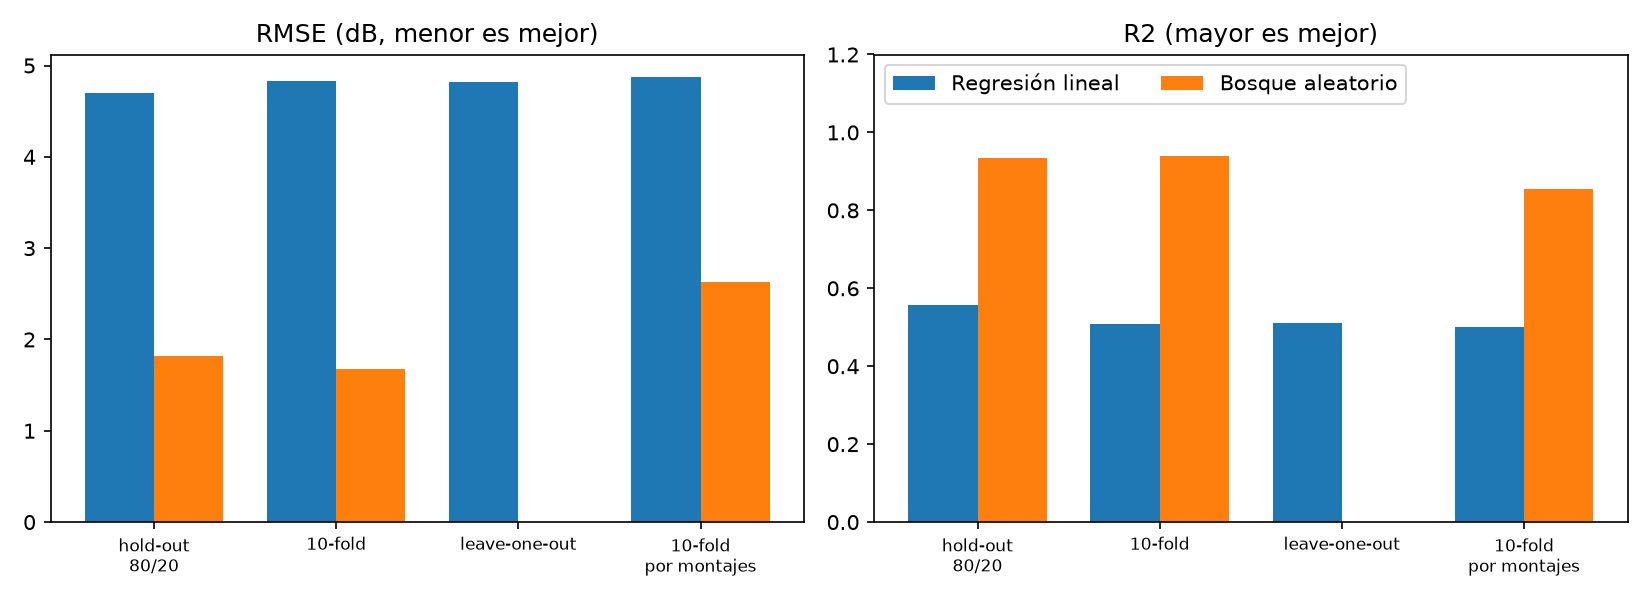
\includegraphics[width=\textwidth]{img/comparacion_metricas.png}
\caption{RMSE y $R^2$ de los dos modelos con cada método de partición. No hay barra del bosque aleatorio con leave-one-out porque no se calculó.}
\label{fig:metricas}
\end{figure}

El bosque aleatorio supera por mucho a la regresión lineal con todas las particiones y todas las métricas. Con 10-fold alcanza $R^2 = 0.941$, MAE de 1.19~dB y RMSE de 1.68~dB, contra $R^2 = 0.509$, MAE de 3.75~dB y RMSE de 4.83~dB de la regresión lineal. Las cuatro métricas ordenan igual a los modelos, pero dicen cosas distintas: el MAE y el RMSE están en decibeles y se interpretan directamente, el MSE está en dB$^2$ y es difícil de interpretar (aunque es la base del RMSE), y el $R^2$ no tiene unidades. El RMSE es mayor que el MAE en los dos modelos (1.68 contra 1.19~dB en el bosque, 4.83 contra 3.75~dB en el lineal) porque eleva al cuadrado los errores y pesa más los grandes, lo que indica que hay predicciones con errores grandes además de los típicos.

Con las particiones aleatorias el resultado es parecido, pero con la partición por montajes el bosque aleatorio empeora de forma notable: el $R^2$ baja de 0.941 a 0.855 y el RMSE sube de 1.68 a 2.63~dB. La regresión lineal casi no cambia (0.509 contra 0.500). La Figura~\ref{fig:metricas} muestra ese contraste.

\subsection{Tarea 3: Análisis de resultados y validez}

El Código~\ref{cod:t5} compara el bosque aleatorio con 10-fold aleatorio y por montajes, grafica los valores reales contra los predichos (Figura~\ref{fig:real}) y genera el reporte automático.

\begin{codigo}[label=cod:t5]{Tarea 3: análisis de resultados y reporte automático}
# El bosque aleatorio es el mejor modelo con la partición aleatoria; se revisa si esa estimación
# se sostiene cuando las pruebas se hacen con montajes que el modelo nunca vio.
print("\n=== Tarea 3: análisis de resultados ===")
nombre = 'Bosque aleatorio'
for particion in ('10-fold', '10-fold por montajes'):
    r = resultados[(nombre, particion)]
    error = reales[(nombre, particion)] - predicciones[(nombre, particion)]
    print(f"{particion}: R2 = {r['R2']:.4f}, RMSE = {r['RMSE']:.3f} dB, "
          f"sesgo medio = {error.mean():.3f} dB, error absoluto p95 = {np.percentile(np.abs(error), 95):.2f} dB")
caida_rmse = resultados[(nombre, '10-fold por montajes')]['RMSE'] / resultados[(nombre, '10-fold')]['RMSE'] - 1
print(f"El RMSE sube {caida_rmse:.1%} al evaluar con montajes no vistos")

fig, ejes = plt.subplots(1, 2, figsize=(11, 4.5), sharex=True, sharey=True)
for eje, particion in zip(ejes, ('10-fold', '10-fold por montajes')):
    eje.scatter(y, predicciones[(nombre, particion)], s=6, alpha=0.5)
    eje.plot([y.min(), y.max()], [y.min(), y.max()], color='tab:red', linestyle='--')
    eje.set_title(f"{nombre}: {particion} (R2 = {resultados[(nombre, particion)]['R2']:.3f})")
    eje.set_xlabel('Presión sonora real (dB)')
ejes[0].set_ylabel('Presión sonora predicha (dB)')
guardar('real_vs_predicho.png')

# Reporte automático: tablas en CSV y resumen en Markdown dentro de resultados/
tabla.round(4).to_csv(os.path.join(CARPETA_RES, 'metricas_por_modelo_y_particion.csv'))
variabilidad.round(4).to_csv(os.path.join(CARPETA_RES, 'variabilidad_particiones.csv'), index=False)
with open(os.path.join(CARPETA_RES, 'reporte_automatico.md'), 'w', encoding='utf-8') as f:
    f.write("# Reporte automático: regresión sobre Airfoil Self-Noise (UCI)\n\n")
    f.write(f"- Instancias: {len(X)}; variables predictoras: {X.shape[1]}; objetivo: presión sonora (dB).\n")
    f.write(f"- Montajes experimentales distintos: {montaje.nunique()} (filas no independientes entre sí).\n")
    f.write("- Modelos: regresión lineal y bosque aleatorio.\n\n")
    f.write("## Métricas por modelo y método de partición\n\n")
    f.write(a_markdown(tabla.round(4)) + "\n\n")
    f.write("## Variabilidad de la estimación según la partición (repeticiones)\n\n")
    f.write(a_markdown(variabilidad.round(4), indice=False) + "\n")
print("\nReporte automático guardado en la carpeta resultados/")
print("Archivos:", sorted(os.listdir(CARPETA_RES)))
\end{codigo}

\begin{consola}[label=out:t5]{Ejecución de \texttt{act22.py}: Tarea 3}
=== Tarea 3: análisis de resultados ===
10-fold: R2 = 0.9407, RMSE = 1.680 dB, sesgo medio = -0.125 dB, error absoluto p95 = 3.47 dB
10-fold por montajes: R2 = 0.8551, RMSE = 2.625 dB, sesgo medio = -0.125 dB, error absoluto p95 = 5.91 dB
El RMSE sube 56.3% al evaluar con montajes no vistos

Reporte automático guardado en la carpeta resultados/
Archivos: ['metricas_por_modelo_y_particion.csv', 'reporte_automatico.md', 'variabilidad_particiones.csv']
\end{consola}

\begin{figure}[htbp]
\centering
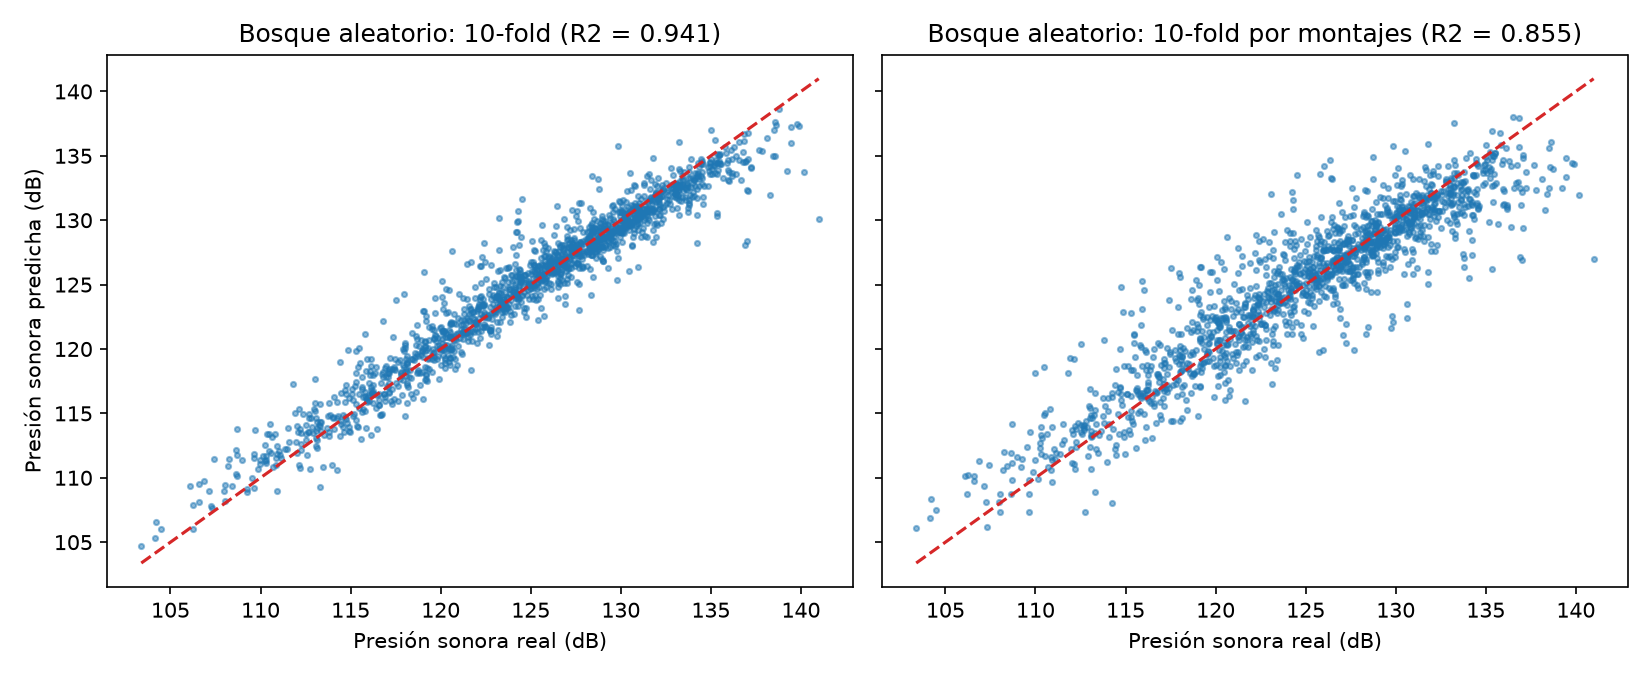
\includegraphics[width=\textwidth]{img/real_vs_predicho.png}
\caption{Presión sonora real contra predicha por el bosque aleatorio. Izquierda: 10-fold aleatorio. Derecha: 10-fold por montajes. La línea punteada es la predicción perfecta.}
\label{fig:real}
\end{figure}

\textbf{Efectividad de las métricas.} Las métricas del tema permitieron comparar los modelos de forma consistente. El $R^2$ muestra de un vistazo que la regresión lineal explica solo la mitad de la variabilidad (0.51) y el bosque casi toda (0.94). El RMSE y el MAE, por estar en decibeles, permiten juzgar si el error es aceptable para la aplicación: con 10-fold, el 95\,\% de los errores absolutos del bosque queda por debajo de 3.5~dB. Un solo número no basta: el $R^2$ alto del bosque por sí solo sugeriría un modelo casi perfecto, y solo al ver el RMSE y el error relativo (24\,\% de la desviación estándar de $y$) se aprecia su alcance. Además, el sesgo medio es casi cero ($-0.13$~dB), por lo que los errores no favorecen una dirección.

\textbf{Efectividad del método de partición.} El hold-out dio una estimación inestable: con una sola partición la regresión lineal obtuvo $R^2 = 0.558$ y el 10-fold dio 0.509, una diferencia que se debe solo a la partición. La validación cruzada de 10 particiones es mucho más estable. Leave-one-out dio prácticamente lo mismo que el 10-fold en la regresión lineal ($R^2$ de 0.511 contra 0.509) con mucho más cómputo, así que no ofrece ventaja con 1503 datos. Lo más importante es que la partición aleatoria (hold-out y 10-fold) no es adecuada para este bosque aleatorio, como se explica a continuación.

\textbf{Punto de vista sobre la validez de los resultados.} Mi opinión es que el resultado de $R^2 = 0.94$ con la validación cruzada aleatoria es demasiado optimista y que el número que debe reportarse es el de la partición por montajes ($R^2 = 0.85$, RMSE de 2.63~dB). La razón es que las filas de un mismo montaje son casi réplicas: comparten ángulo, cuerda, velocidad y espesor y solo cambian en la frecuencia. Con una partición aleatoria, un montaje tiene filas en entrenamiento y en prueba, y el bosque aleatorio, que puede memorizar, predice bien una fila ya vista casi por completo. Es una fuga de información entre entrenamiento y prueba, y coincide con la advertencia del tema de que en estos métodos no se puede garantizar la independencia de los datos \parencite{tecnm2026_tema33}. La regresión lineal no sufre el problema porque no puede memorizar, y por eso su métrica casi no cambia.

Qué estimación es la correcta depende de la pregunta. Si el modelo se usara para predecir el ruido de montajes ya medidos a otras frecuencias, la validación aleatoria sería razonable. Si se usara para diseñar un perfil nuevo, que es el uso natural, la correcta es la partición por montajes, y entonces se debe esperar un error típico de 2.6~dB, con un 5\,\% de los errores por encima de 5.9~dB. Aun así, hay límites en lo que se puede afirmar: los resultados son de un solo conjunto de datos y de una sola semilla, no se ajustaron los hiperparámetros del bosque, los 106 montajes son pocos para estimar con precisión el desempeño en montajes nuevos y no se calcularon intervalos de confianza. Tampoco deben compararse los valores de los folds con pruebas paramétricas, porque no son independientes \parencite{tecnm2026_tema33}.

\subsection{Reporte automático}

Al terminar, el script guarda en la carpeta \texttt{resultados/} el archivo \texttt{metricas\_por\_modelo\_y\_particion.csv} (MAE, MSE, RMSE, $R^2$ y error relativo de cada combinación), \texttt{variabilidad\_particiones.csv} (resultados de las repeticiones de la Tarea 1a) y \texttt{reporte\_automatico.md}, un resumen con la descripción del conjunto, los montajes distintos y las dos tablas. Las figuras de este reporte se generan en \texttt{img/}. Para analizar otro conjunto de regresión basta con cambiar la sección de datos y, si existen grupos de filas relacionadas, la definición de los grupos.

\section{Conclusiones}

El bosque aleatorio predice la presión sonora mucho mejor que la regresión lineal con las cuatro métricas del tema: con validación cruzada de 10 particiones obtiene $R^2 = 0.941$ y RMSE de 1.68~dB, contra 0.509 y 4.83~dB. Las métricas coinciden en el orden de los modelos y se complementan: el RMSE y el MAE dan el error en decibeles y el $R^2$ lo relativiza respecto de la variabilidad de los datos.

La principal lección es sobre la partición. El hold-out resultó inestable y leave-one-out no aportó nada con 1503 datos, mientras que la validación cruzada de 10 particiones fue estable. Pero como las filas de un mismo montaje no son independientes, la partición aleatoria infla el desempeño del bosque aleatorio, y al probar con montajes no vistos el $R^2$ baja de 0.94 a 0.85 y el RMSE sube 56\,\%. Un resultado de validación solo es confiable si la partición refleja cómo se usará el modelo; aquí, el valor que debe reportarse es el de la partición por montajes.

\referencias

\end{document}
